%\section{The Tour}
Tempo player is an application for the Android platform, which is able to play and select music from an already existing library of songs, which fits the user's running pace measured in steps per minute (SPM). It uses the accelerometer for calculating the user's running pace. The application's main screen can be seen in \Cref{fig:mainScreen}. 

\begin{figure}[h!]
  \centering
    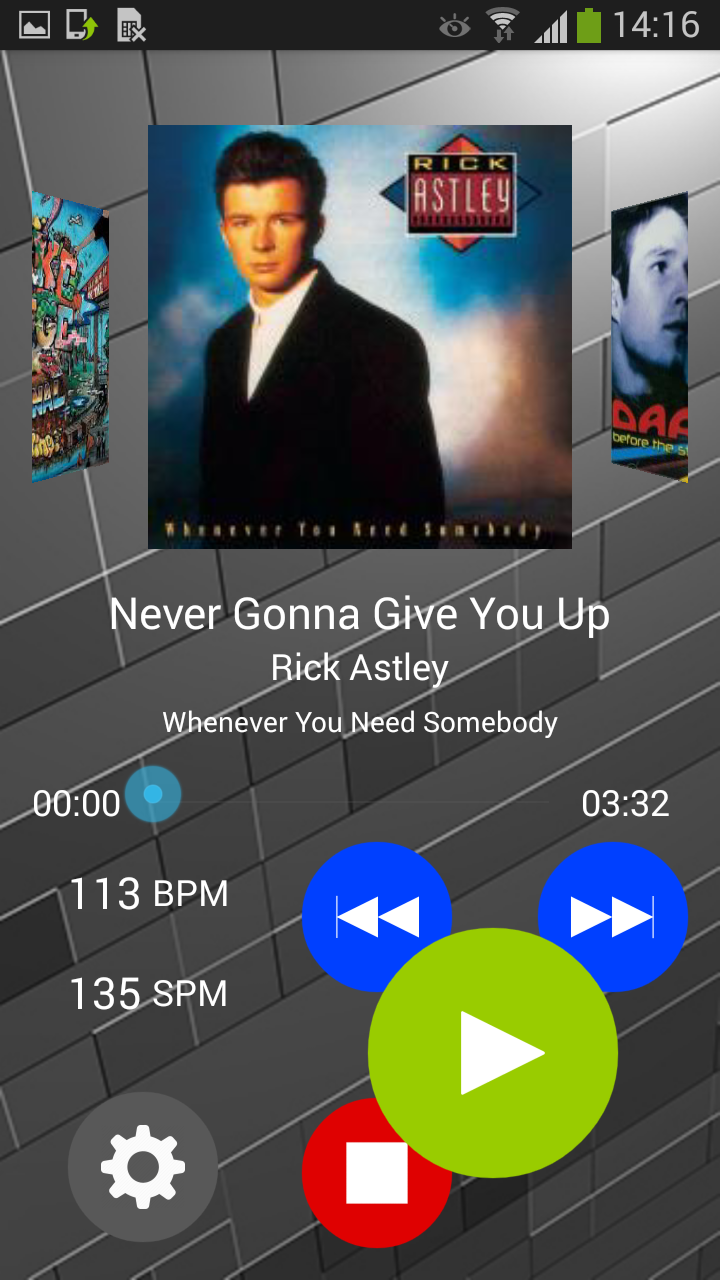
\includegraphics[scale=0.2]{Images/Screenshots/mainScreen.png}
  \caption{A screenshot showing Tempo Player's main screen.}
  \label{fig:mainScreen}
\end{figure}

The \textit{BPM} represent the song's ``Beats Per Minute''. This information is retrieved from a web service and therefore the application initially requires an internet connection to function as intended. After the songs' BPMs are retrieved, they are stored in an SQL Lite database for later use. The \textit{SPM} represent the user's current number of steps per minute.

The Android device should be mounted on the user's arm and when the next button is pressed the BPM of the next songs played will match the user's SPM if possible, otherwise nearest BPM is selected.

When the user stands still for more than 2 seconds, the SPM are set to 0, since no steps are taken. See \Cref{sec:stepCnt} for details. 

When standing still all songs in the library will be available to the user in a shuffled order. \Alexander{Sure?}

As shown in \Cref{fig:settings}, the user can adjust some settings of the application. Currently, the only adjustment the user can make is in which directory the application looks for songs. This settings screen is shown in \Cref{fig:settingsPath}. 

It is also possible to seek to a position in the currently playing song by dragging the seek bar to a location along the time line. 

%This chapter should describe an overview of the program, as well as provide a couple of screenshots detailing the GUI of the program.

%i.e. Tempo Player is a music player that utilises the accelerometer to count the steps of the user. 
%Tempo Player then compares this pace with the beats per minute of songs collected in a SQL Lite database, and plays the one most similar. 
%The beats per minutes of each song are found by querying a web service. 
\begin{figure}
\centering
\begin{minipage}{.5\textwidth}
  \centering
    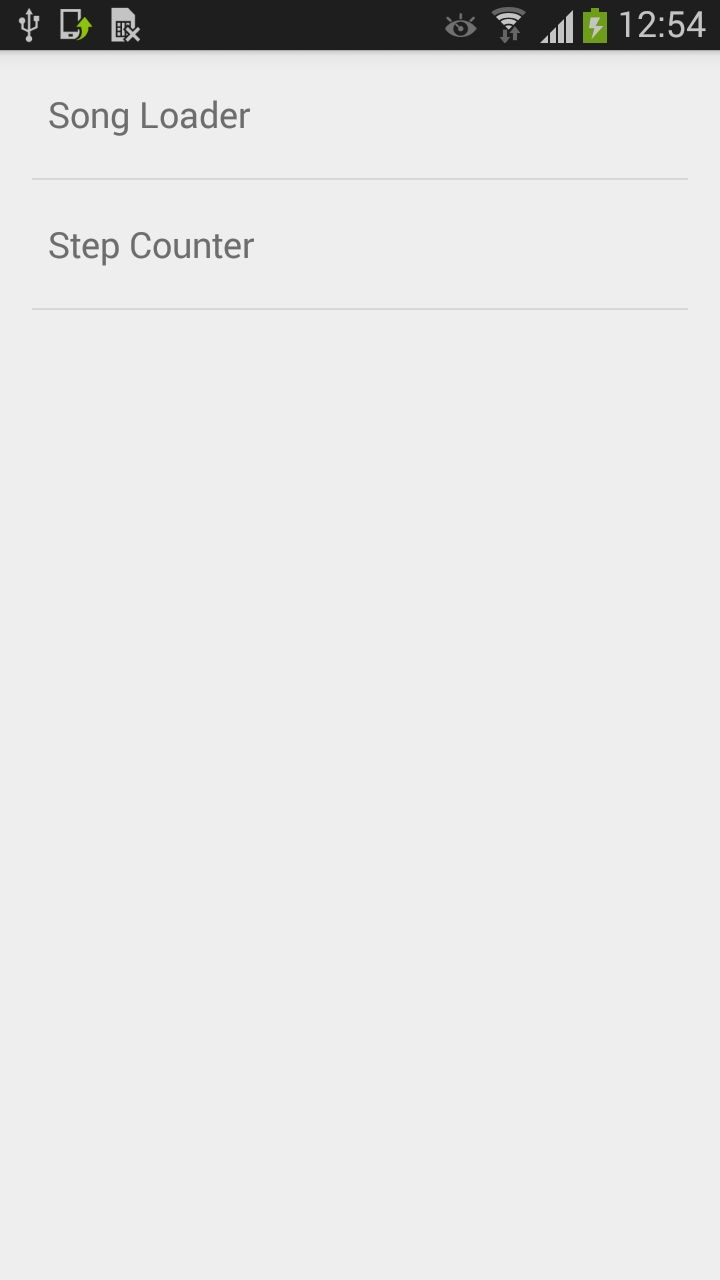
\includegraphics[scale=0.2]{Images/Screenshots/settings.png}
  \caption{Screenshot showing the \newline settings screen.}
  \label{fig:settings}
\end{minipage}%
\begin{minipage}{.5\textwidth}
\centering
    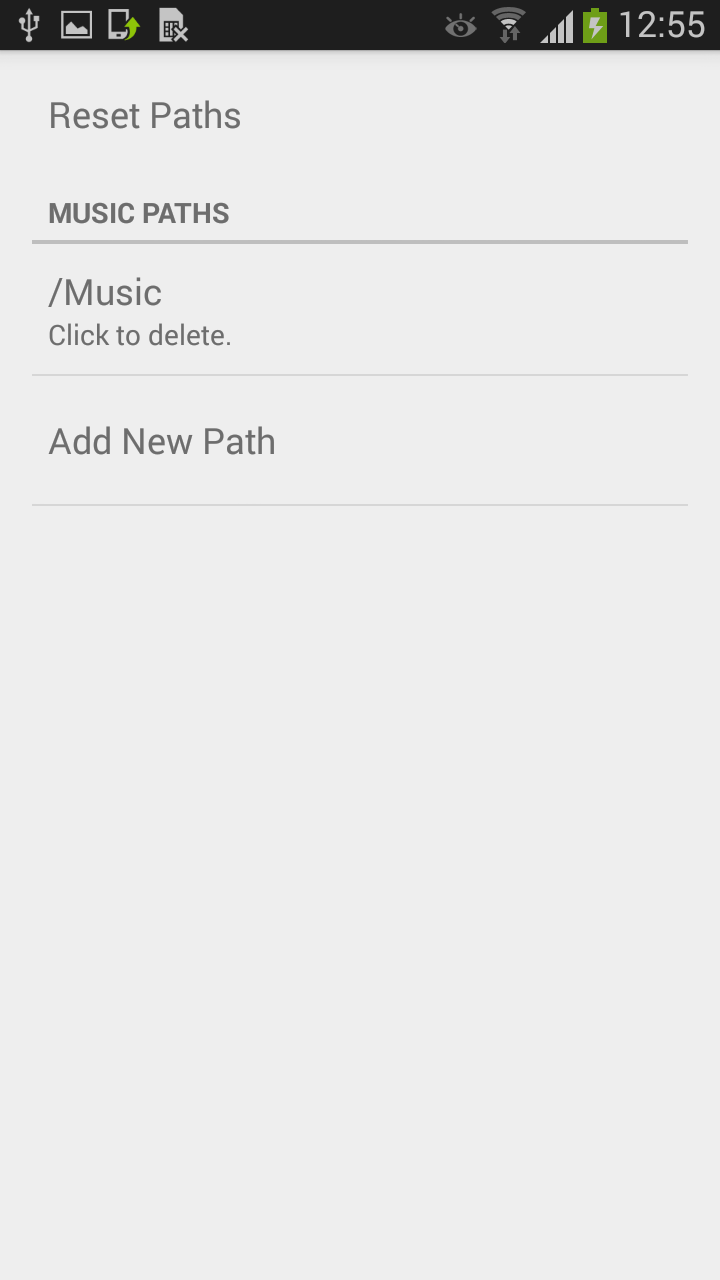
\includegraphics[scale=0.2]{Images/Screenshots/settingsPath.png}
  \caption{Screenshot showing the ``Reset paths'' screen of the settings screen.}
  \label{fig:settingsPath}
\end{minipage}
\end{figure}